\documentclass[../ManualeSviluppatore.tex]{subfiles}

\begin{document}
\section{Mappatura edificio}
	Nella presente sezione si vuole fornire una descrizione della soluzione implementata per effettuare \gls{navigazione indoor}.
	
	Per \textbf{mappatura edificio} si intende la costruzione teorica di un \textbf{grafo pesato} che rappresenta l'edificio in cui abilitare la funzionalità di navigazione offerta dall'applicazione.
	
	Per un edificio quindi è necessario individuare i due elementi che compongono un grafo:
	\begin{itemize}
		\item Vertici;
		\item Archi.
	\end{itemize}
	
	\subsection{Vertici: Region of Interest e Point of Interest}
	
	I \textbf{vertici} rappresentano le aree coperte dal segnale di un singolo \gls{beacon}, definite Region Of Interest (\gls{ROI}).
	Ogni ROI, identificata da un unico \gls{beacon}, è definita come un insieme di possibili destinazioni da raggiungere all'interno dell'edificio da mappare. Tali destinazioni sono definite Point Of Interest (\gls{POI}) e rappresentano nella realtà tutti i punti di interesse di un utente.
	
	\begin{figure} [h]
		\centering
		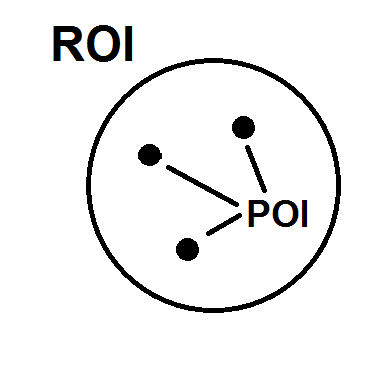
\includegraphics[scale=0.4]{img/ROIePOI}
		\caption{Visione teorica di ROI e POI contenuti in essa}
		\label{fig:ROIePOI}
	\end{figure}
	
	Una ROI e quindi un \gls{beacon}, rappresenta più POI per soddisfare gli obiettivi di \textbf{massimizzare l'area da coprire} e \textbf{minimizzare il numero di beacon} da utilizzare.
	
	Poiché è possibile che un POI abbia più punti d'accesso (si pensi ad una stanza con più porte d'accesso) è previsto che un singolo POI possa appartenere a più ROI. Il risultato è una relazione N a N tra ROI e POI. Nella figura \ref{fig:ROIePOI-NtoN} si illustra graficamente come un POI possa appartenere a più ROI, nel caso rappresentato il POI al centro appartiene sia alla ROI$_1$ sia alla ROI$_2$.
	
	\begin{figure} [h]
		\centering
		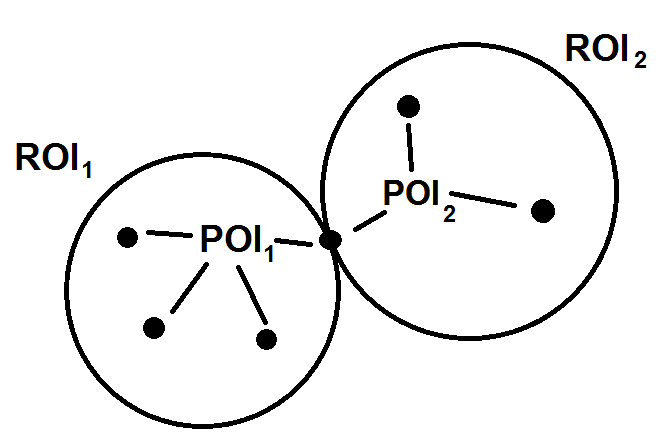
\includegraphics[scale=0.4]{img/POIeROI-NtoN}
		\caption{Visione teorica di un POI che appartiene a più ROI}
		\label{fig:ROIePOI-NtoN}
	\end{figure}
	
	
	\subsection{Gli archi: Edge}
	
	Gli \textbf{archi} (Edge) invece rappresentano i collegamenti reali tra una ROI e un'altra ROI, per esempio un corridoio o delle scale.
	Essi quindi possono essere di varie tipologie e quindi pesati in modo diverso. Le tipologie fin'ora individuate sono:
	\begin{itemize}
		\item Default Edge;
		\item Stair Edge;
		\item Elevator Edge.
	\end{itemize}
	Ogni Edge contiene le informazioni necessarie per arrivare correttamente alla ROI di arrivo dalla ROI di partenza.
	
	
	\subsection{Percorso}
	Un POI è una possibile destinazione dell'utente ossia il punto d'arrivo di un possibile percorso mentre una ROI è l'area in cui l'utente si trova, grazie al rilevamento dei \gls{beacon}. Gli Edge e i ROI tra queste due entità rappresentano il percorso da percorrere.
	
	Dato quindi un punto di partenza e uno di arrivo abbiamo la necessità di calcolare il percorso più corto per raggiungere il punto di arrivo. Poiché lavoriamo identificando gli spazi interni dell'edificio con elementi di un grafo, possiamo sfruttare tutta la conoscenza matematica su questi.
	Implementando l'algoritmo di Dijkstra otteniamo il percorso più corto da una ROI ad un'altra.
	
	Poiché il punto di destinazione è un POI e questo può appartenere a diverse ROI nel calcolo del percorso bisogna identificare il percorso migliore tra la ROI di partenza e le ROI di cui il POI fa parte.

	
	
	\subsection{Mappare più piani}
	
		Se consideriamo ogni piano di un edificio come un grafo possiamo connettere tali grafi con nuovi Edge nei punti reali in cui questi piani si collegano, scale e ascensori. Otteniamo così da due grafi un grafo più grande.
		
		\begin{figure} [h]
			\centering
			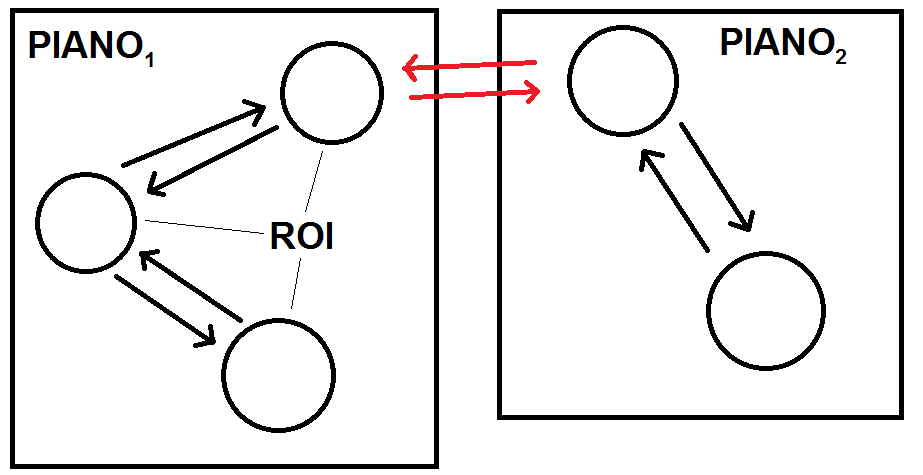
\includegraphics[scale=0.4]{img/GRAFI-CONNESSI}
			\caption{Visione teorica di un collegamento tra due grafi ossia piani di un edificio}
			\label{fig:GRAFI-CONNESSI}
	\end{figure}
	
		
	\subsection{Configurazione beacon}
		Per gestire questa soluzione teorica i beacon fanno da ROI del grafico ossia i vertici. La scelta della loro posizione è di fondamentale importanza per il corretto funzionamento della navigazione e della user experience. 

		I dati trasmessi dal \gls{beacon} sono il Major e il Minor, ovvero due stringhe composte da cinque caratteri numerici. Nella soluzione presentata sono così utilizzati:
		\begin{description}
			\item[Major:] identificativo dell'edificio supportato dall'applicazione;
			\item[Minor:] le prime due cifre identificano il piano mentre le ultime tre la ROI.
		\end{description}			
		
		Di seguito si elencano quali sono le pratiche da seguire individuate dal team \leaf\ per ottenere un risultato ottimale:
		\begin{itemize}
			\item gli spazi interni dell'edificio devono essere il più possibile coperti dal segnale dei \gls{beacon} evitando il più possibile sovrapposizioni tra questi;
			\item ogni ROI e quindi ogni \gls{beacon} si consiglia di posizionarlo in tutti gli incroci di un edificio e nei luoghi di accesso di ogni stanza o punto di interesse (POI);
			\item il collegamento reale (Edge teoricamente) tra due ROI deve essere il più possibile una linea retta. L'applicazione infatti calcola alcune indicazioni da dare sulla base della coordinata magnetica/orientamento da una ROI ad un altro;
		\end{itemize}


	\subsection{Procedura per la mappatura di un edificio}
		Nel caso si volesse che l'applicazione CLIPS supporti un altro edificio seguire questi passaggi:
		\begin{enumerate}
			\item procurarsi una planimetria dell'edificio;
			\item identificare tutti i POI dell'edificio di ogni piano;
			\item raggruppare i POI vicini in ROI garantendo che:
			\begin{itemize}
				\item tutto l'edificio sia coperto dal segnale dei beacon;
				\item non ci sia eccessiva distanza tra una ROI e un'altra;
				%\item una ROI non contenga troppi POI;
			\end{itemize}
			\item collegare ogni ROI alle ROI raggiungibili da essa senza passare per altre ROI e identificando la tipologia di Edge (normale, scale, ascensori\dots). \textbf{NOTA:} se da un ROI posso raggiungere un'altra ROI e viceversa dovrò necessariamente documentare due Edge distinti.
			\item per ogni Edge identificato rilevare le informazioni necessarie per descriverlo in toto:
			\begin{itemize}
				\item distanza;
				\item coordinata magnetica;
				\item azione che l'utente deve seguire;
				\item descrizione dettagliata;
				\item ROI di partenza;
				\item ROI di fine;
			\end{itemize}
			Tali informazioni saranno fondamentali perché l'applicazione offra il maggior numero di informazioni all'utente;
			\item assegnare ai \gls{beacon} da utilizzare un Major univoco che identifica l'edificio che si sta mappando;
			\item assegnare ad ogni \gls{beacon} un Minor in cui le prime due cifre identificano il numero del piano e le ultime tre identificano la ROI in quel piano;
			\item inserire nel server delle mappe tali informazioni. Per ulteriori informazioni su quest'ultimo punto si rimanda alla sezione \ref{sec:PersistenzaDeiDati}.
		\end{enumerate}
		
	\subsection{Area sviluppatore}
	Nell'applicazione è stata inclusa un'\textbf{area sviluppatore} accessibile solo tramite password. Tale area ha lo scopo di facilitare la raccolta di dati e mostrarli tramite l'interfaccia grafica dell'applicazione. È stato fatto ciò per consentire di effettuare più facilmente e velocemente test sul campo durante la \textbf{mappatura di un edificio}. Di seguito si elencano i passaggi necessari per accedervi e le funzionalità offerte:
	\begin{enumerate}
		\item dal menu dell'applicazione selezionare \textbf{Area sviluppatore};
		\item inserire il codice sviluppatore sottostante:
		\begin{quote}
			\centering
			\verb|miriade|
		\end{quote}
		\item effettuare l'operazione desiderata:
		\begin{itemize}
			\item visualizzazione dettagliata dei log salvati;
			\item avvio di un nuovo log;
			\item rimozione di un log salvato.
		\end{itemize}
	\end{enumerate}		
	
	Per approfondire le possibilità offerte da tale funzionalità si rimanda alla consultazione del \textit{Manuale Utente}.

\end{document}